\setcounter{chapter}{4}
\setcounter{section}{0}
\setcounter{figure}{0}
\setcounter{equation}{0}
\setcounter{table}{0}
\chapter*{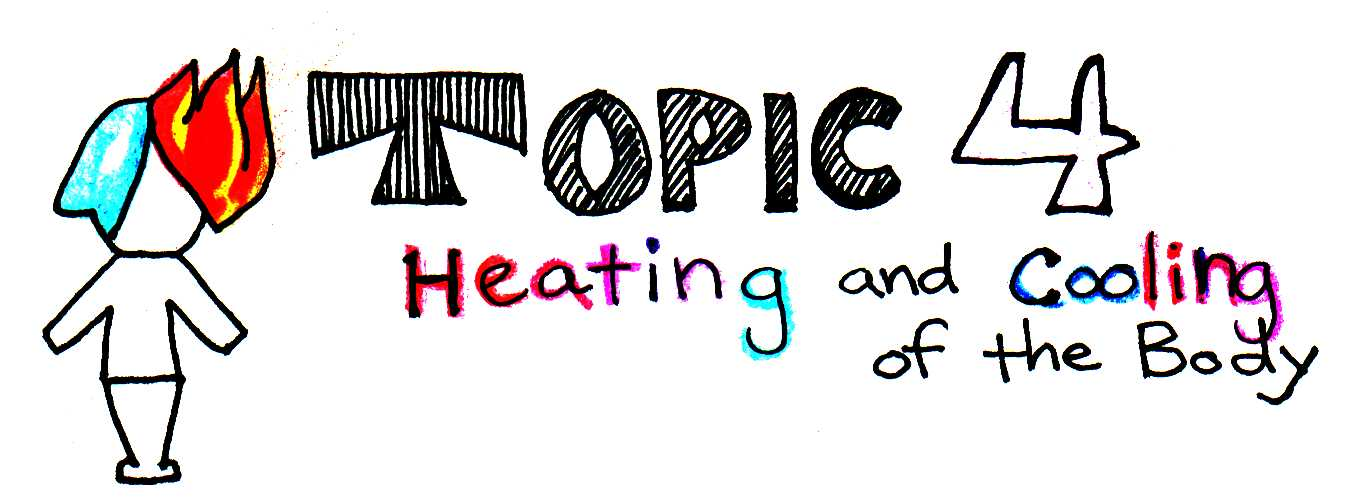
\includegraphics[width=\textwidth]{./figures/Topic4/Topic4.jpg}}
\addcontentsline{toc}{chapter}{Topic 4: Heating and Cooling of the Body}

\section{Introduction}

Thermoregulation is the maintenance of body temperature within a range at which cells can function effectively.  Although various species have adapted differently, each is suited to an optimal temperature range.  Each animal has physical and behavioral adaptations that allow it to maintain a constant internal temperature, regardless of fluctuations in the ambient (external) temperature.  
Body temperature on the skin’s surface is much lower than the temperature of tissues deep inside the body -- the so-called ``core temperature.''  For humans, the core temperature is normally between 98$^{\circ}$F and 98.6$^{\circ}$F (measured orally).  Even when exposed for several hours to ambient temperatures between 60$^{\circ}$F and 130$^{\circ}$F, our core temperature varies little -- from 97$^{\circ}$F to 100$^{\circ}$F.  Figure \ref{Fig4-1} illustrates this stability of the core temperature.
\begin{figure}[h]
	\centering
	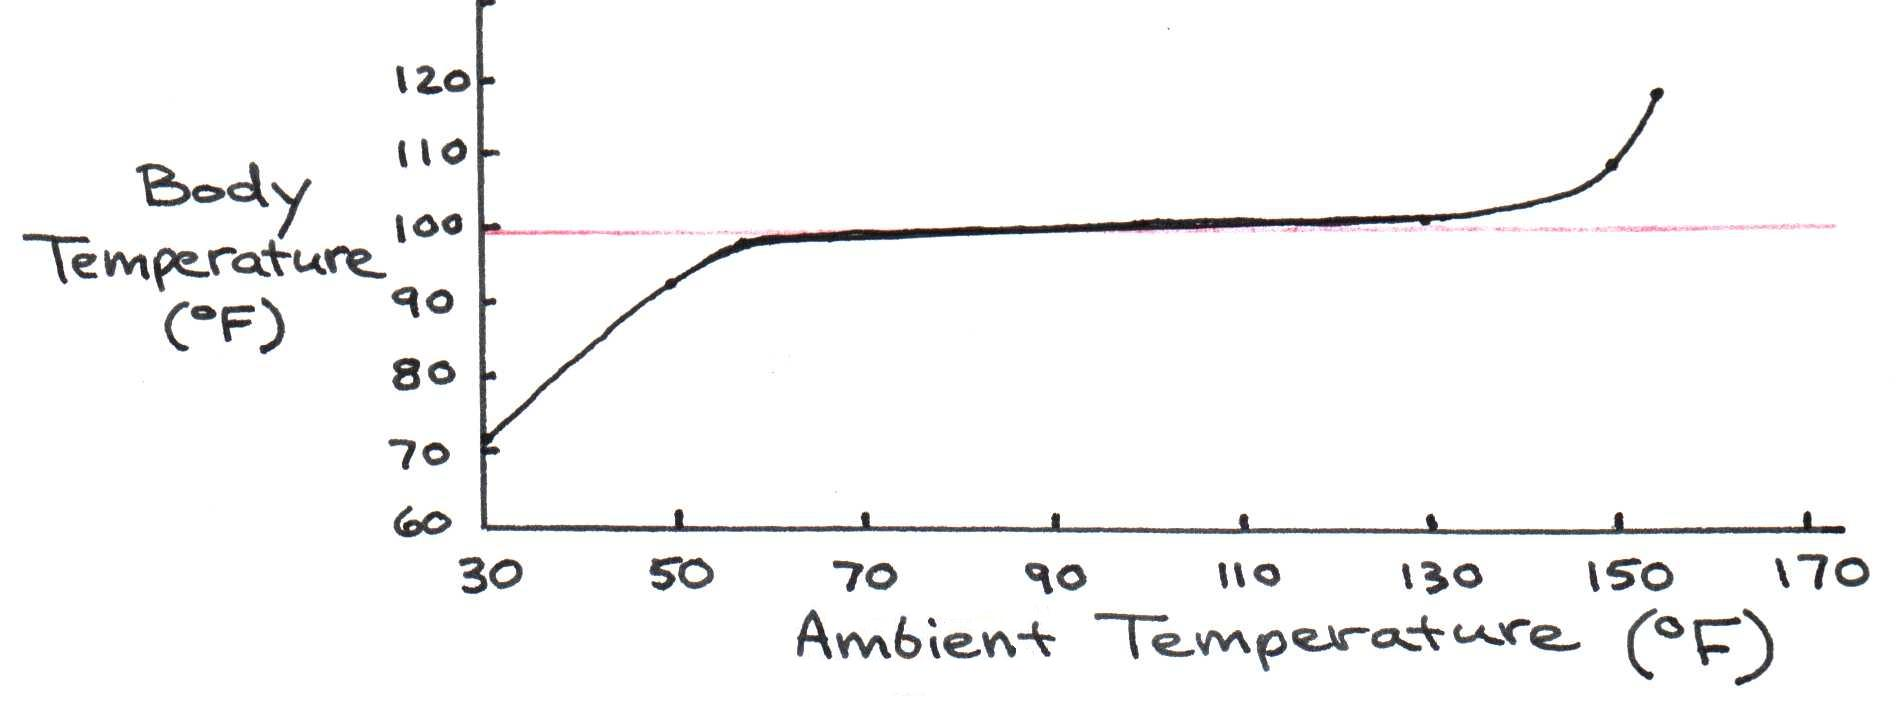
\includegraphics[width=\textwidth]{./figures/Topic4/Fig4-1.jpg}
	\caption{Effect of ambient temperature on internal body temperature.  Note the stability of the core temperature despite wide variations in atmospheric temperature.}
	\label{Fig4-1}
\end{figure}  

How do we accomplish thermoregulation?  A portion of our brain known as the hypothalamus controls a number of mechanisms that balance heat production with heat dissipation.  We will first discuss how heat is produced through metabolic activity and then investigate the ways in which heat is dissipated into the environment.
  
\section{Heat Production}

Unlike cold-blooded animals (ectotherms), which warm their bodies by absorbing heat from their environment, humans and other endotherms generate heat from chemical reactions in the body.  These chemical reactions (see Appendix B), collectively referred to as metabolism, are generally inefficient, releasing over 75\% of their energy as heat.
 
This internal generation of heat is particularly noticeable during fever, which is a natural immune response to invading pathogens. When the hypothalamus receives chemical signals characteristic of invading pathogens it increases metabolism, which is partially responsible for the increased temperature of the body. Metabolism also increases during strenuous exercise.  As muscles work hard, cells require more energy and thus must increase their rate of respiration.  Cellular respiration is the process of using oxygen and complex food molecules to create ATP, a molecule often dubbed the cell’s ``energy currency.''  So much internal heat is created from these reactions that under moderate ambient temperatures, the core temperatures can rise to 102$^{\circ}$F or 103$^{\circ}$F.  In hot weather, the core temperature can rise to a dangerous 106-108$^{\circ}$F during exercise.
The basal metabolic rate (BMR) for an endotherm is defined as the baseline rate of metabolism with no muscle activity, on an empty stomach, and with no stress.  Many factors can influence the BMR, including age, sex, body size, body temperature, ambient temperature, quality and quantity of food, and activity level.  For humans, the average BMR is approximately 60 kcal/hour for young adult males and 53 kcal/hour for young adult females.  (While we often speak of “counting calories,” the amounts of energy listed on nutritional information labels are actually measured in kilocalories, where 1 kilocalorie (kcal or C) = 1,000 calories.  Also, 1 kcal = 4,186 J.  Just to maintain the BMR, males must consume 1,600-1,800 kcal per day and females must consume 1,300-1,500 kcal per day.  Eating and digesting increases daily caloric expenditure by 200 kcal, while sitting adds another 200 kcal.  Depending on the level of activity, work done by muscles requires an even greater energy intake.  A laborer can expend up to 7,000 kcal per day, and some Olympic athletes as much as 12,000 kcal per day.

\section{Heat Dissipation}

The core temperature is controlled by balancing heat production with several heat loss mechanisms.  Three physical processes serve to remove heat from the body:
\begin{itemize}
\item Radiation ($\sim$60\%)
\item Evaporation ($\sim$20\%)
\item Conduction ($\sim$20\%)
\end{itemize}
The percentages listed are rough estimates of how much each process contributes to the overall heat loss of the body. These percentages may vary considerably depending on what clothes you wear, how humid the air is. 
In this section, we will briefly discuss the physical principles behind each of these heat loss mechanisms before moving on to how the body uses them to regulate temperature.

\subsection{Radiation}

Radiation accounts for about 60\% of the body’s total heat loss.  All bodies emit energy in the form of electromagnetic radiation.  People and objects give off waves with different wavelengths and intensities, depending on their temperature.  Humans emit waves in the infrared part of the electromagnetic spectrum.  Infrared goggles allow users to see the ``glow'' emitted by living creatures by detecting these waves and converting them to visible ones.  
The total power emitted by a body is given by  the Stefan-Boltzmann law,
\begin{equation}\label{eqn4-1}
P = A\epsilon\sigma T^4,
\end{equation}
where $A$ is the body’s surface area, $\epsilon$ is the emissivity constant, $\sigma$ is the Stefan-Boltzmann constant ($\sigma$ = 5.67$\times 10^{-8}$ W/m$^2\cdot$K$^4$), and $T$ is the body’s absolute temperature.  The emissivity constant e is a dimensionless quantity between 0 and 1 that measures how close the body comes to radiating like an ``ideal'' body, one that absorbs all radiation incident upon it.

Because all bodies (animate or inanimate) emit radiation, the human body absorbs radiation emitted by other bodies in its environment.  Thus, rather than finding the total power emitted by a body, we are more interested in knowing the net rate of radiation from a body (emitted – absorbed).  If the body has temperature T in an environment with temperature TAmbient, the net power emitted is given by the following equation:
\begin{equation}\label{eqn4-2}
P_{radiation} = A\epsilon \sigma \left(T^4-T_{ambient}^4\right)
\end{equation}
For a human being, $\epsilon \approx$ 1 and $A \approx$ 1.2 m$^2$.  For a normal body temperature of 33$^{\circ}$C and an ambient temperature of 22$^{\circ}$C, $T$ = 306 K and $T_{ambient}$ = 295 K.  Using these values, the net power dissipation by the average adult human is 81 W.  This is about 2/3 of the power produced by metabolism for a resting adult who burns 100 kcal/hour, or 120 W.  Note that positive values for $P_{net}$ indicate that radiation is emitted by the body, whereas negative values indicate absorption by the body of radiation from the environment.
  
\subsection{Evaporation}

Heat is also lost through the evaporation of water from skin and through breathing.  The rate of heat loss due to evaporation depends on the rate of evaporation, which in turn depends on the humidity of the air.  If the air is saturated with moisture (100\% humidity), no evaporation can take place.  If, instead, the air is dry (0\% humidity), the evaporation rate reaches a maximum.  
To vaporize 1 g of water at room temperature (25$^{\circ}$C), 0.58 kcal heat must be transferred to the water. The energy to evaporate water is the latent heat of vaporization. As shown in Fig.~\ref{Fig4-2}, at the surface temperature of the body ($T$ = 306 K) the heat of vaporization is $L \approx 2400$ kJ/kg.
\begin{figure}[h]
	\centering
	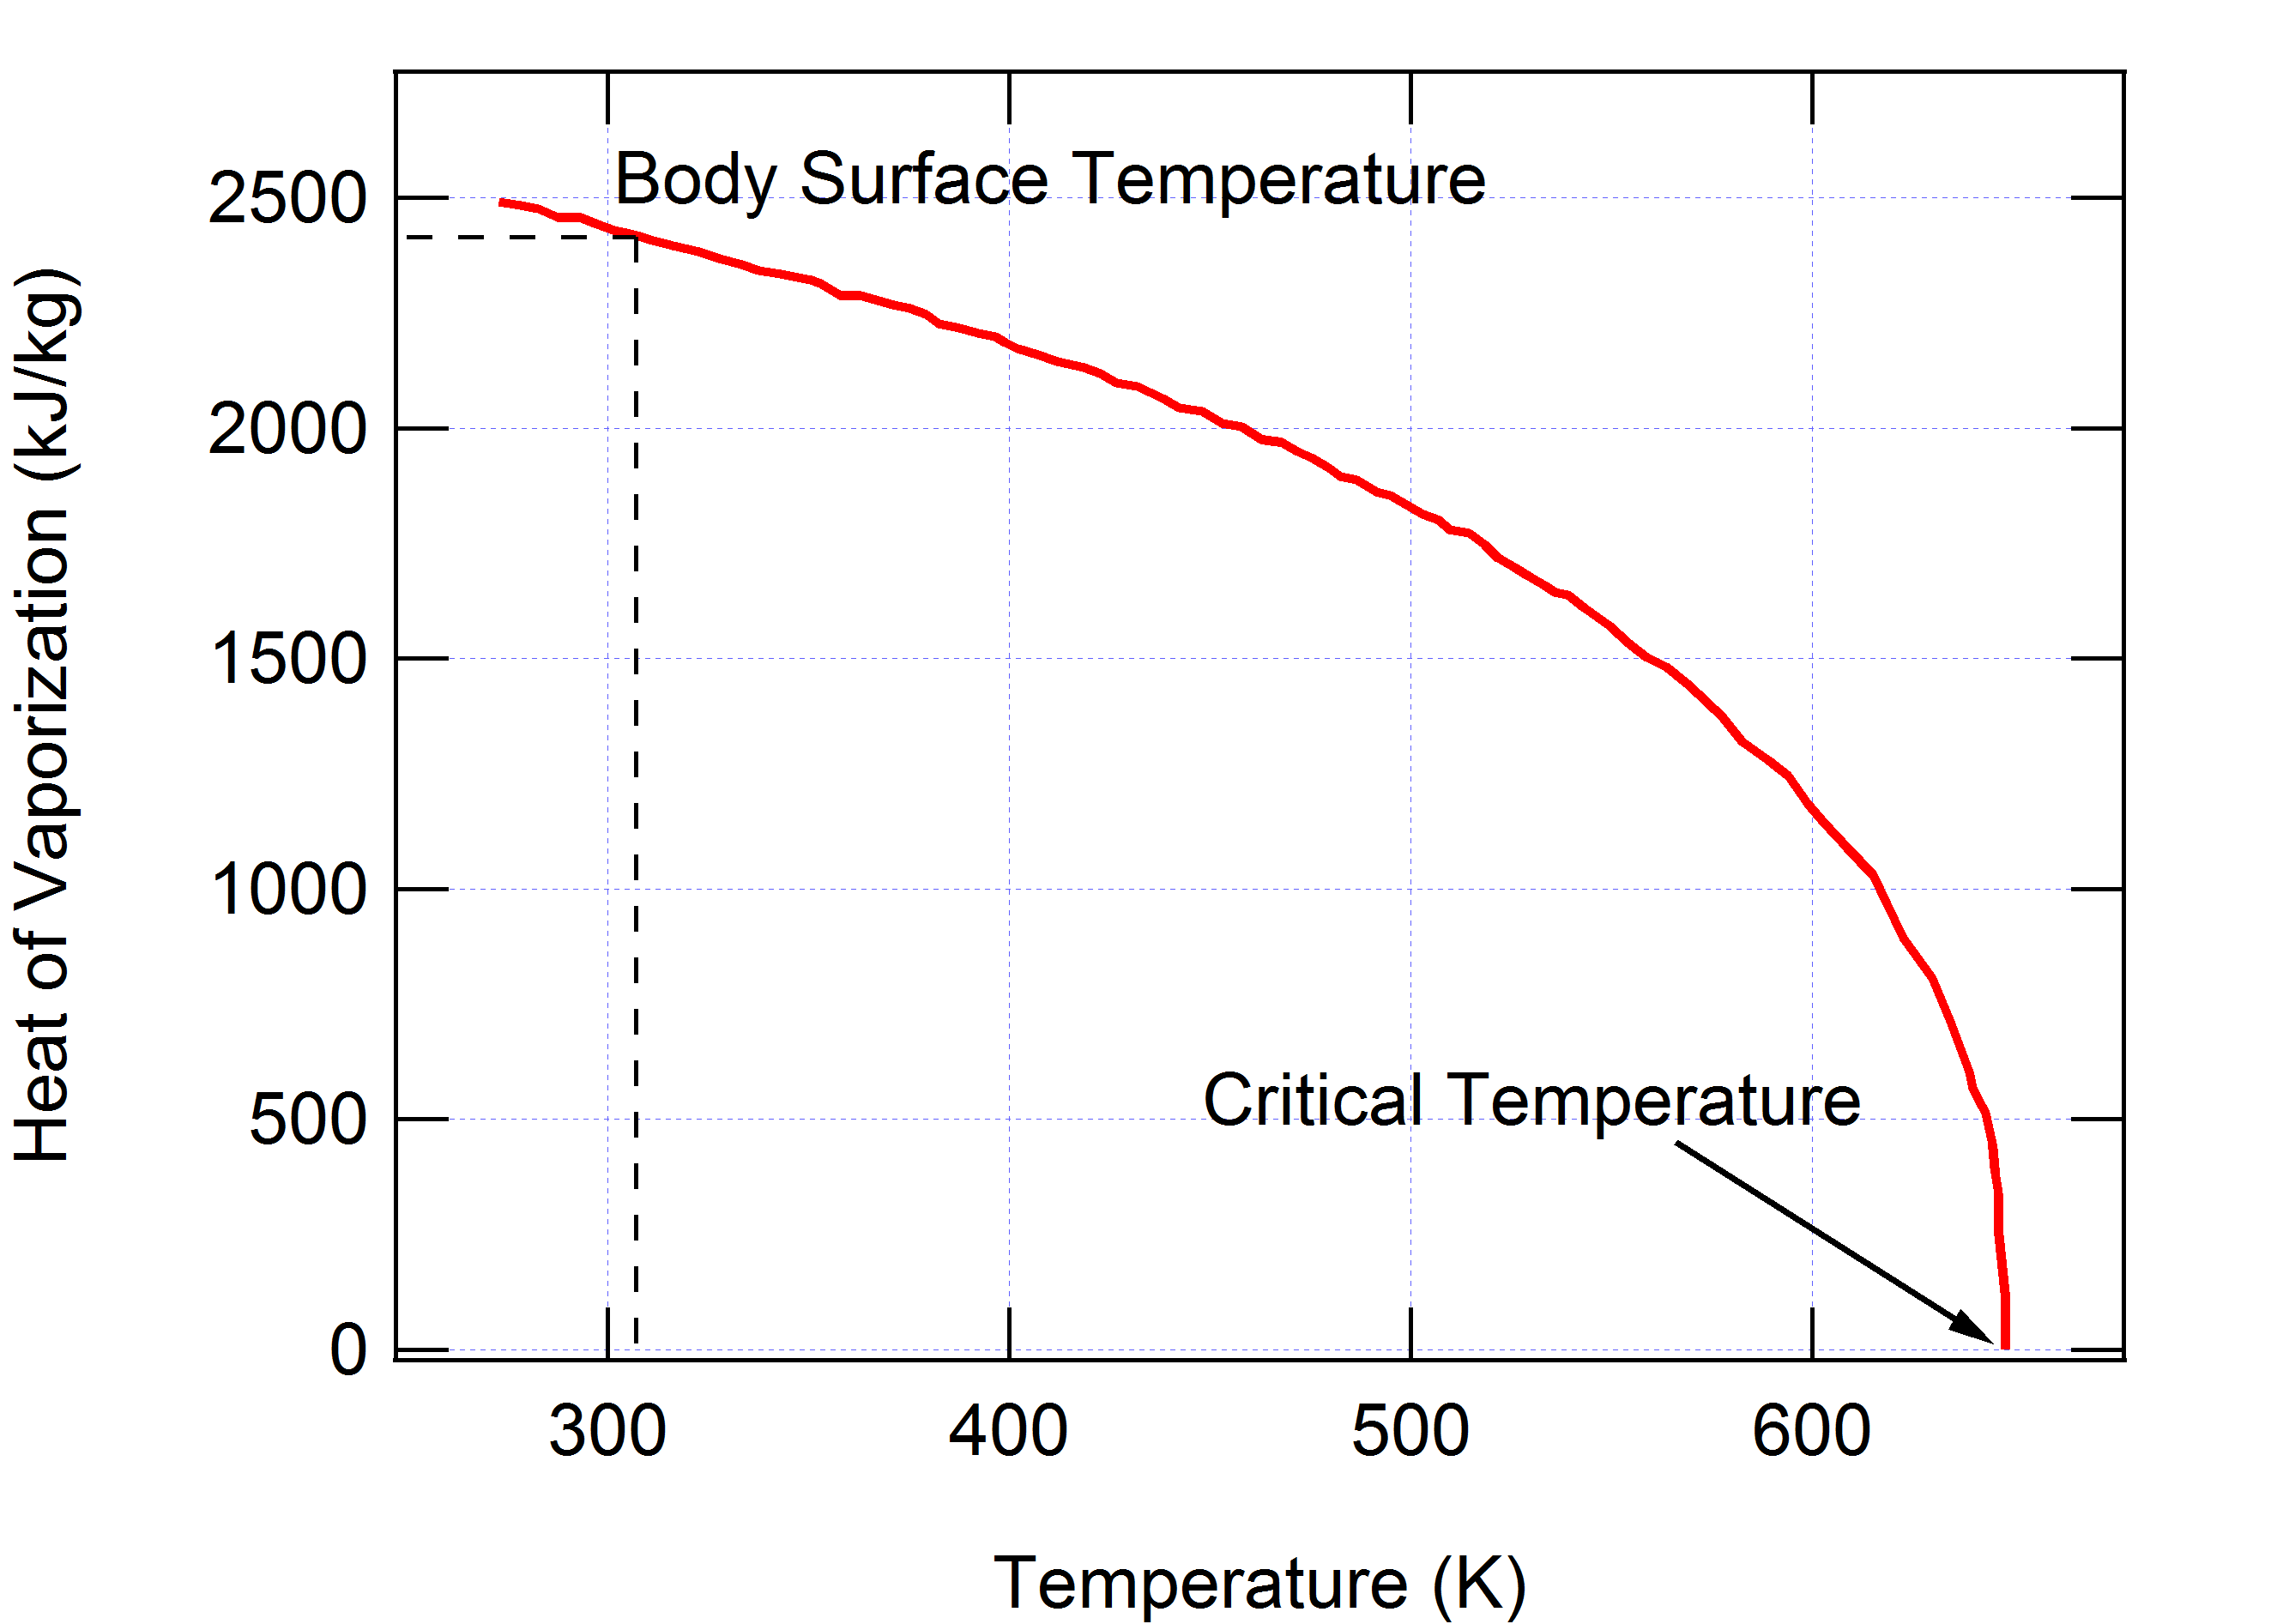
\includegraphics[width=\textwidth]{./figures/Topic4/Fig4-2.png}
	\caption{The heat required to evaporate water at temperatures ranging from freezing to the critical point above which only the gaseous phase of water exists.}
	\label{Fig4-2}
\end{figure}
Without sweating, the average person loses about 0.6 liters of water per day due to evaporation, equivalent to a cooling rate of 15 kcal/hour, or 18 W.  Under extreme conditions and for acclimatized persons, a body can lose as much as two liters of water per hour.  At this rate, the person will cool at a rate of 1,160 kcal per hour, equivalent to 1300 W, by sweating alone!

\subsection{Conduction}

Conduction refers to heat transfer within a body or between two bodies in contact.  Heat always moves from areas of high temperature towards areas of low temperatures.  Typically, the human body is warmer than its environment, so heat moves from the body to surrounding air or to objects in contact with our skin.  The power dissipated from our skin to the environment is governed by the equation
\begin{equation}\label{eqn4-3}
P_{conduction} = \frac{kA\left(T-T_{ambient}\right)}{d}
\end{equation}
where $k$ is the conductivity of air ($k$ = 0.024 W/m$\cdot$K) and $d$ represents the thickness of the insulating layer or air that surrounds the body ($d\approx$ 1 cm with clothes and 0.3 cm without).  Using the $d$ value for clothing and the values used previously for $A$, $T$, and $T_{ambient}$, the heat loss due to conduction is about 33 W.

\section{Regulation of Body Temperature}

As stated before, body temperature is regulated by an area of the brain called the hypothalamus.  Heat sensors in the skin and throughout the body respond to temperature changes by stimulating the hypothalamus to evoke certain responses.  These responses are described below.    

\subsection{Responses to High Temperatures}

\subsubsection{Vasodilation}
Along with nutrients, blood carries heat.  Blood circulating deep within the body picks up heat, which can be subsequently carried by the circulation to the skin.  There the heat is dissipated into the environment and the cooled blood re-enters the body ready to transfer more heat.  Our bodies possess a heat sensing mechanism that regulates blood flow to the skin in relation to the need for heat dissipation. The blood flow is regulated by a network of blood vessels underneath the skin that contract or dilate as needed. For instance, these blood vessels dilate as the body’s temperature rises above the optimal range to divert greater blood flow to the skin. As much as one-third of the cardiac output can be rerouted so that heat can be removed from the body.  The effectiveness of this mechanism is demonstrated in Fig.~\ref{Fig4-3}, which shows how much heat conduction from the core to the skin takes place as the ambient temperature rises.  
\begin{figure}[h]
	\centering
	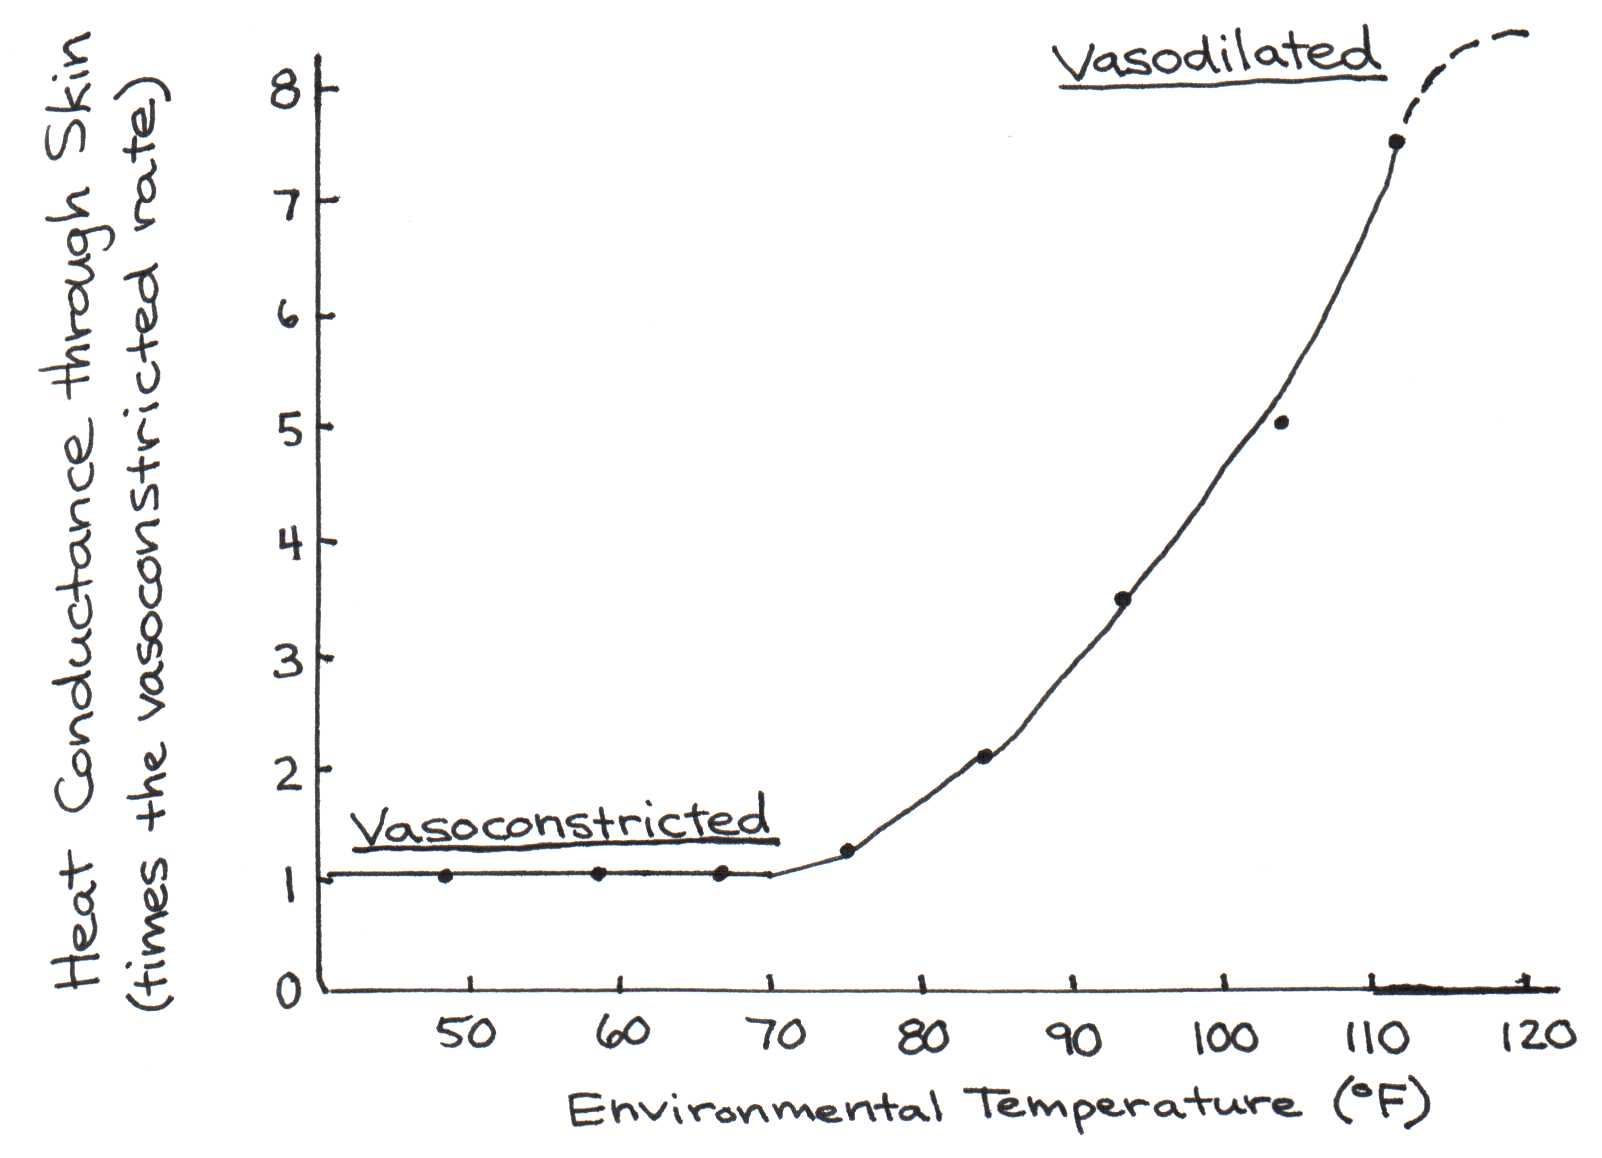
\includegraphics[width=\textwidth]{./figures/Topic4/Fig4-3.jpg}
	\caption{Effect of ambient temperature changes on heat conductance from the body core to the skin surface.  At 110$^{\circ}$F, the skin loses seven times as much heat through the skin because of vasodilation.}
	\label{Fig4-3}
\end{figure}
  
\subsubsection{Sweating and Behavioral Cooling}

As already discussed, sweating is the predominant form of evaporative cooling.  Many animals that do not sweat, like dogs and birds, pant to increase evaporative cooling in their mouths and throats.  Since a wet body surface can be 50--100 times more effective at conducting heat than a dry one, most animals also find relief from the hot sun by bathing in cold water.  A cold beverage on a warm day really does cool you down-heat from your core is transmitted to the liquid, making you less hot.

\subsubsection{Reduction of Metabolism}

A third way to reduce heat is to reduce the amount of metabolic activity going on inside the body.  The hypothalamus sends signals to other parts of the brain that control chemical pathways, telling them to slow down.  

\subsection{Responses to Low Temperatures}

\subsubsection{Vasoconstriction}

Vasoconstriction on the skin is exactly the opposite of vasodilation—heat is retained in the core by limiting the blood flow near cooler regions, like the skin.  Many marine animals and endotherms have adapted a counter-current heat exchanger, a unique arrangement of blood vessels that allows heat to pass from the warmer blood in the arteries to the cooler blood in the veins, minimizing heat loss outside of the body.  

\subsubsection{Piloerection}

Recall from Eq.~\ref{eqn4-2} the inverse relation between $d$, the thickness of air insulating the body, and the power dissipated by the body.  Many animals can trap more insulating air around the skin by fluffing up fur or feathers.  This method of decreasing heat loss is called piloerection.  Goose bumps are an evolutionary throwback to a time when our more hairy ancestors made use of this ability.

\subsubsection{Increased Heat Production}

Shivering, the increased contraction of muscles, produces heat in the body.  Alternatively,  hormones can trigger cellular metabolism to produce heat instead of ATP.  This is called nonshivering thermogenesis.  Both of these processes actually produce more heat rather than simply preventing heat from escaping the body.    

